\section{Account erstellen}

Auf der Account erstellen Seite ist es möglich seinen eigenen Account zu erstellen. Hierzu wird ein 
einfaches HTML-Formular verwendet, welches bei \textit{submit} die eingegeben Daten an den Server sendet,
als sowohl auch den Benutzer direkt einloggt. Existiert allerdings bereits ein User mit selben Namen 
beziehungsweise selbe Email, wird die Meldung \textit{dieser Benutzer existiert bereits} ausgegeben. Um 
Tippfehler beim Passwort zu vermeiden, existiert ein Passwort bestätigen Feld. Die Überprüfung ob die
Passwort bestätigen Zeichenkette die selbe ist wie die Passwort Zeichenkette erfolgt über die 
JavaScript Bibliothek \textbf{Yup} von \textit{monastic.panic}.

\begin{figure}[H]
    \begin{center}
      \frame{\includegraphics[width=1\textwidth]{Website/Passwörter-dont-match.png}}
      \caption{Fehlermeldung für nicht Übereinstimmende Passwörter}
    \end{center}
\end{figure}
\pagebreak

Um eine höhere Sicherheit zu garantieren, muss das Passwort mehr als sechs Zeichen beinhalten. Die 
Fehlermeldung für ein zu kurzes Passwort würde wie folgt aussehen.

\begin{figure}[H]
    \begin{center}
      \frame{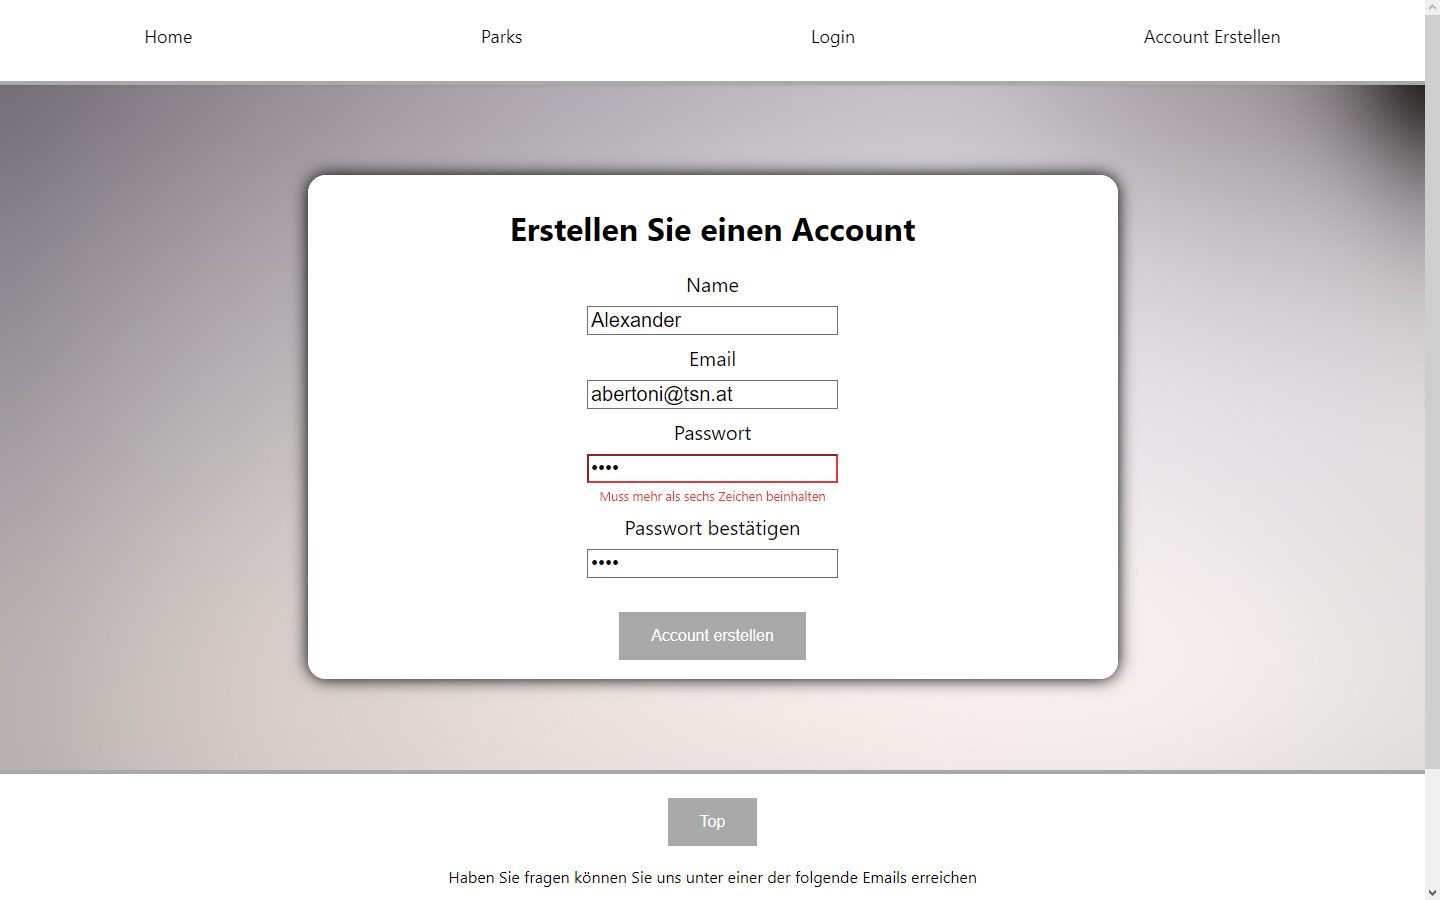
\includegraphics[width=1\textwidth]{Website/Passwort-zu-kurz.png}}
      \caption{Fehlermeldung für nicht Übereinstimmende Passwörter}
    \end{center}
\end{figure}


\label{createAccount}